% !Mode:: "TeX:UTF-8"
% !TEX program  = xelatex
\documentclass[a4paper]{article}
\usepackage{amsmath}
\usepackage{amssymb}
\usepackage{ctex}
%\usepackage{braket}
\usepackage[european]{circuitikz}
\usepackage{multirow}
\usepackage{float}
\usepackage{url}
%\usepackage[table,xcdraw]{xcolor}
\usepackage{colortbl}
\usepackage{geometry}
\geometry{left=2.5cm,right=2.5cm,bottom=2.5cm,top=2.5cm}
\title{模电实验报告7:积分与微分电路实验}
\author{xy\quad 学号\quad 匡亚明学院}
\date{2019年2月29日}
\begin{document}
\maketitle
\bibliographystyle{unsrt}
%--------main-body------------

\section{实验目的}
\begin{enumerate}
\item 学习使用运放组成积分与微分电路。
\end{enumerate}

\section{实验仪器}
示波器、信号发生器、交流毫伏表、数字万用表。

\section{预习内容}
\begin{enumerate}
\item 阅读OP07的“数据手册”,了解OP07的性能。
\item 复习关于积分与微分电路的理论知识。
\item 阅读本次实验的教材。
\end{enumerate}

\section{实验内容}
\subsection{积分电路}
积分电路如图(\ref{intcd})所示。
\begin{figure}[!h]
\centering
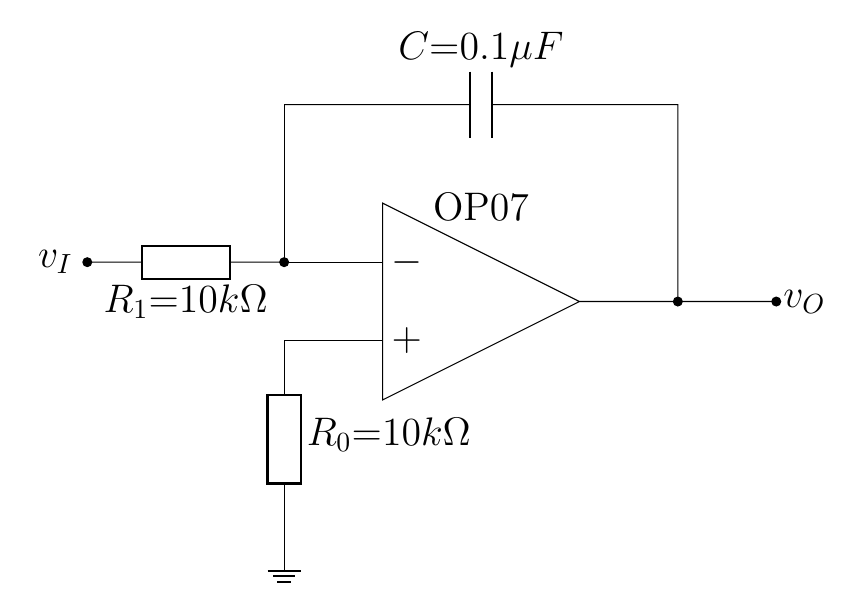
\begin{tikzpicture}[x=2.5cm,y=2.5cm]
\draw (0,0.2) to [short, *-] (0,1);
%----C-----------------------------------------
\draw (0,1) to [C, l =\Large $C{=}0.1\mu F$] (2,1) to [short, -*] (2,0) to [short,-*] (2.5,0);
%-----------R_0--------------------------------
\draw (0,-0.2) to [R, l =\Large $R_0{=}10k\Omega$] (0,-1.2) to node[ground](GND){} (0,-1.2);
\draw (0,-0.2) -- (0.5,-0.2);
\draw (0,0.2) -- (0.5,0.2);
%----------draw the opamp----------------------
\draw (1.5,0) -- (0.5,0.5) -- (0.5,-0.5) -- (1.5,0) -- (2,0);
\draw (0,0.2) to [R, l =\Large $R_1{=}10k\Omega$, -*] (-1,0.2);
%----------text--------------------------------
\draw (-1.3,0.2) node[anchor = west]{\Large $v_I$}
    (0.75,0.2) node[anchor=east]{\Large $-$}
    (0.75,-0.2) node[anchor=east]{\Large $+$}
    (1,0.6) node[anchor = north]{\Large OP07}
    (2.8,0) node[anchor=east]{\Large $v_O$};
\end{tikzpicture}
\caption{积分电路}\label{intcd}
\end{figure}

在理想条件下,
\begin{equation}
\cfrac{v_I(t)}{R_1} = -C\cfrac{\text{d}v_O(t)}{\text{d}t}
\end{equation}
当C两端的初始电压为零时,则
\begin{equation}
v_O(t) = -\cfrac{1}{R_1C}\int^{t}_{0}v_I(t)\text{d}t
\end{equation}
因此得名积分电路。
\subsubsection{测量积分电路幅频特性曲线}
取C=0.1$\mu$F,测量积分电路的幅频特性曲线。观察输入输出的波形。测量得到的幅频特性数据填入表(\ref{int_AFC_table})。
\subsubsection{改进的积分电路的方波波形}
使用如图(\ref{intcd})所示的电路进行实验,通常会观察到输出的直流漂移,解决办法是在电容C两端并联一个电阻$R_2$,改进的积分电路如图(\ref{intcd_s}):
\begin{figure}[!h]
\centering
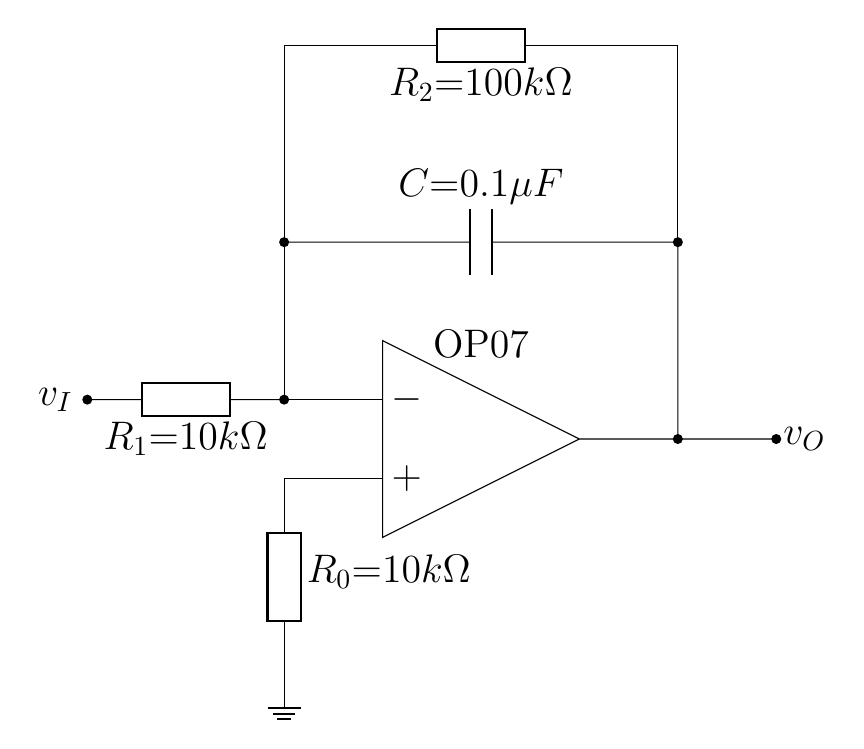
\begin{tikzpicture}[x=2.5cm,y=2.5cm]
\draw (0,0.2) to [short, *-] (0,1);
%----C-----------------------------------------
\draw (0,1) to [C, l =\Large $C{=}0.1\mu F$] (2,1) to [short, -*] (2,0) to [short,-*] (2.5,0);
%-------R_2------------------------------------
\draw (0,1) to [short,*-] (0,2) to [R,l_ =\Large $R_2{=}100k\Omega$] (2,2) to [short,-*] (2,1);
%-----------R_0--------------------------------
\draw (0,-0.2) to [R, l =\Large $R_0{=}10k\Omega$] (0,-1.2) to node[ground](GND){} (0,-1.2);
\draw (0,-0.2) -- (0.5,-0.2);
\draw (0,0.2) -- (0.5,0.2);
%----------draw the opamp----------------------
\draw (1.5,0) -- (0.5,0.5) -- (0.5,-0.5) -- (1.5,0) -- (2,0);
\draw (0,0.2) to [R, l =\Large $R_1{=}10k\Omega$, -*] (-1,0.2);
%----------text--------------------------------
\draw (-1.3,0.2) node[anchor = west]{\Large $v_I$}
    (0.75,0.2) node[anchor=east]{\Large $-$}
    (0.75,-0.2) node[anchor=east]{\Large $+$}
    (1,0.6) node[anchor = north]{\Large OP07}
    (2.8,0) node[anchor=east]{\Large $v_O$};
\end{tikzpicture}
\caption{直流闭环的积分电路一阶低通滤波器}\label{intcd_s}
\end{figure}

取输入信号的峰峰值为1V,频率分别为20Hz,1kHz,2kHz,记录所得的输入输出波形图。

\subsection{微分电路}
\subsubsection{测量微分电路的幅频特性曲线}
按图(\ref{diffcd_s})连接电路,测量幅频特性数据填入表(\ref{diff_AFC_table})。
\begin{figure}[!h]
\centering
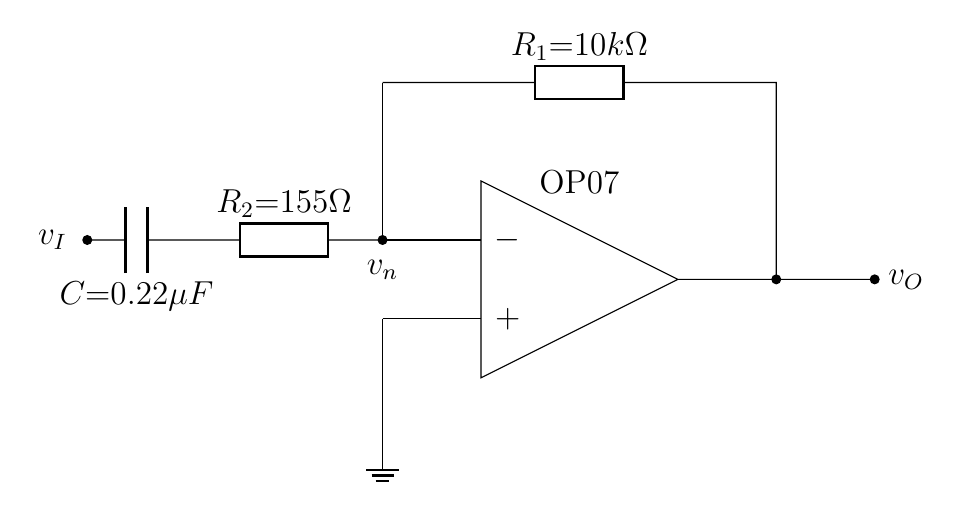
\begin{tikzpicture}[x=2.5cm,y=2.5cm]
\draw (0,0.2) to [short, *-] (0,1);
%----R_1----------------------------------------
\draw (0,1) to [R, l =\large $R_1{=}10k\Omega$] (2,1) to [short, -*] (2,0) to [short,-*] (2.5,0);
%-----------R_0--------------------------------
\draw (0,-0.2) to (0,-0.8) node[ground]{};
\draw (0,-0.2) -- (0.5,-0.2);
\draw (0,0.2) -- (0.5,0.2);
%----------draw the opamp----------------------
\draw (1.5,0) -- (0.5,0.5) -- (0.5,-0.5) -- (1.5,0) -- (2,0);
%-------R_2------------------------------------
\draw (0,0.2) to [R, l_ =\large $R_2{=}155\Omega$] (-1,0.2)
    (-1,0.2) to [C,l =\large $C{=}0.22\mu F$,-*] (-1.5,0.2);
%----------text--------------------------------
\draw (-1.8,0.2) node[anchor = west]{\large $v_I$}
    (0,-0.05) node[anchor = south]{\large $v_n$}
    (0.75,0.2) node[anchor=east]{\large $-$}
    (0.75,-0.2) node[anchor=east]{\large $+$}
    (1,0.6) node[anchor = north]{\large OP07}
    (2.8,0) node[anchor=east]{\large $v_O$};
\end{tikzpicture}
\caption{微分电路优化设计}\label{diffcd_s}
\end{figure}
\subsubsection{改进的微分电路的方波波形}
取输入信号峰峰值为0.2V,频率分别为10Hz,100Hz,1kHz,观察输入输出波形。

\subsection{积分-微分电路}
按图(\ref{int-diff-cd})连接电路,改变输入信号频率从10Hz到10kHz,记录积分-微分电路的幅频特性数据,填表。
\begin{figure}[!h]
\centering
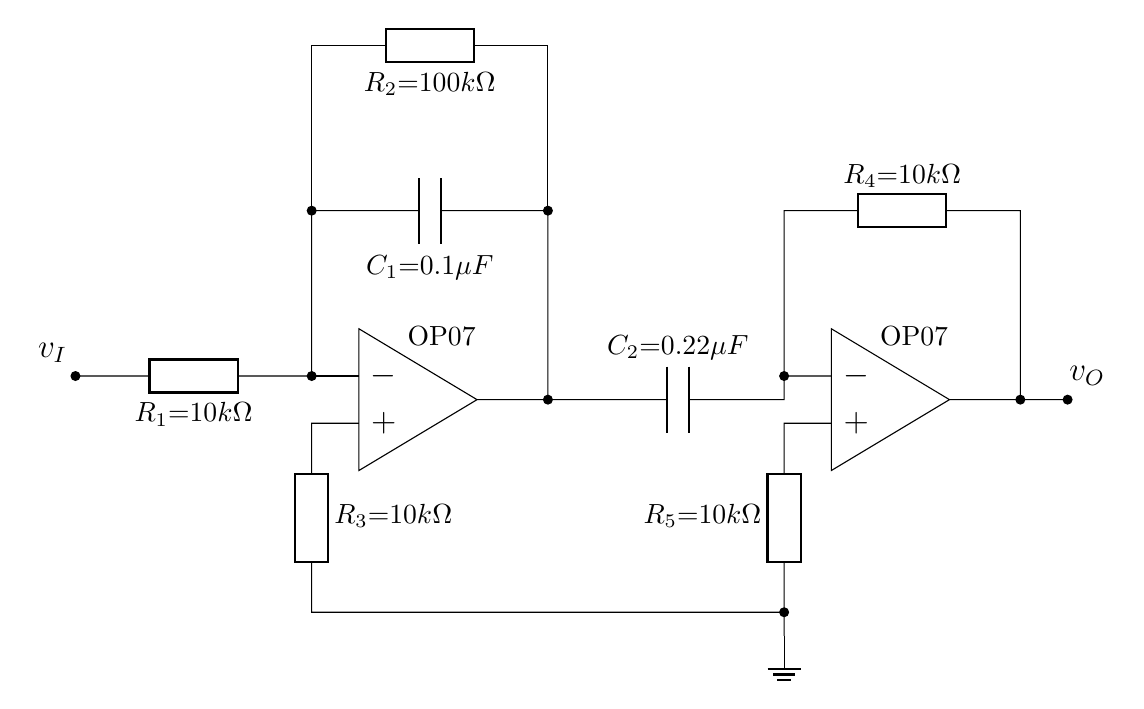
\begin{tikzpicture}[x=3cm,y=3cm]
\draw (0,-0.1) to [short,*-*] (0,0.7) to [C,l = $C_1{=}0.1\mu F$] (-1,0.7) to [short,*-*] (-1,0) to [R, l = $R_1{=}10k\Omega$,-*] (-2,0);
\draw (0,0.7) -- (0,1.4) to [R,l = $R_2{=}100k\Omega$] (-1,1.4) -- (-1,0.7);
%---OP07_1-------------------------------------------
\draw (-0.3,-0.1) -- (-0.8,0.2) -- (-0.8,-0.4) -- (-0.3,-0.1) -- (0.5,-0.1) to [C,l = $C_2{=}0.22\mu F$] (0.6,-0.1) -- (1,-0.1) -- (1,0) -- (1.2,0);
%---OP07_2-------------------------------------------
\draw (1.7,-0.1) -- (1.2,0.2) -- (1.2,-0.4) -- (1.7,-0.1) -- (2,-0.1) to [short,*-*] (2.2,-0.1);
\draw (-1,0) -- (-0.8,0);
\draw (-0.8,-0.2) -- (-1,-0.2) to [R,l = $R_3{=}10k\Omega$] (-1,-1) -- (1,-1) -- (1,-1.1) node[ground]{};
\draw (1,-1) to [R,l = $R_5{=}10k\Omega$,*-] (1,-0.2) -- (1.2,-0.2);
%------R_4-------------------------------------
\draw (1,0) to [short, *-] (1,0.7) to [R,l = $R_4{=}10k\Omega$] (2,0.7) -- (2,-0.1);
%----------text--------------------------------
\draw (-2.2,0.1) node[anchor = west]{\large $v_I$}
    (-0.6,0) node[anchor=east]{\large $-$}
    (-0.6,-0.2) node[anchor=east]{\large $+$}
    (1.4,0) node[anchor=east]{\large $-$}
    (1.4,-0.2) node[anchor=east]{\large $+$}
    (-0.45,0.25) node[anchor = north]{OP07}
    (1.55,0.25) node[anchor = north]{OP07}
    (2.4,0) node[anchor=east]{\large $v_O$};
\end{tikzpicture}
\caption{积分--微分电路}\label{int-diff-cd}
\end{figure}

图(\ref{int-diff-cd})中的电阻$R_2$的作用为防止直流漂移,电容$C_2$旁缺少的155$\Omega$电阻会使得幅频特性曲线中出现一个突变的峰。

\section{实验数据}
\subsection{积分电路}
取输入信号为$v_{ipp}$=1.03V的正弦波。
\subsubsection{积分电路幅频特性}
积分电路的幅频特性数据如表(\ref{int_AFC_table}):
\begin{table}[!h]
\centering
\caption{积分电路幅频响应}
\label{int_AFC_table}
\begin{tabular}{|c|c|c|c|c|c|c|c|c|}
\hline
\rowcolor[HTML]{EFEFEF} 
$f_i$/Hz                     & 10   & 20   & 30  & 40   & 50   & 60    & 70    & 80   \\ \hline
$v_{opp}$/V              & 13.8 & 6.9  & 4.6 & 3.5  & 2.8  & 2.3   & 2.0   & 1.7  \\ \hline
$v_o(\text{幅值}=\frac{v_{opp}}{2})$/V & 6.9  & 3.45 & 2.3 & 1.75 & 1.4  & 1.15  & 1.0   & 0.85 \\ \hline
\rowcolor[HTML]{EFEFEF} 
$f_i$/Hz                     & 90   & 100  & 150 & 200  & 300  & 500   & 1000  & 5000 \\ \hline
$v_{opp})$/V              & 1.6  & 1.4  & 1.0 & 0.7  & 0.5  & 0.29  & 0.15  & 0.1  \\ \hline
$v_o(\text{幅值}=\frac{v_{opp}}{2})$/V & 0.8  & 0.7  & 0.5 & 0.35 & 0.25 & 0.145 & 0.075 & 0.05 \\ \hline
\end{tabular}
\end{table}

根据表(\ref{int_AFC_table})画出幅频特性曲线,如图(\ref{AFC_int_fig}):
\begin{figure}[!h]
\centering
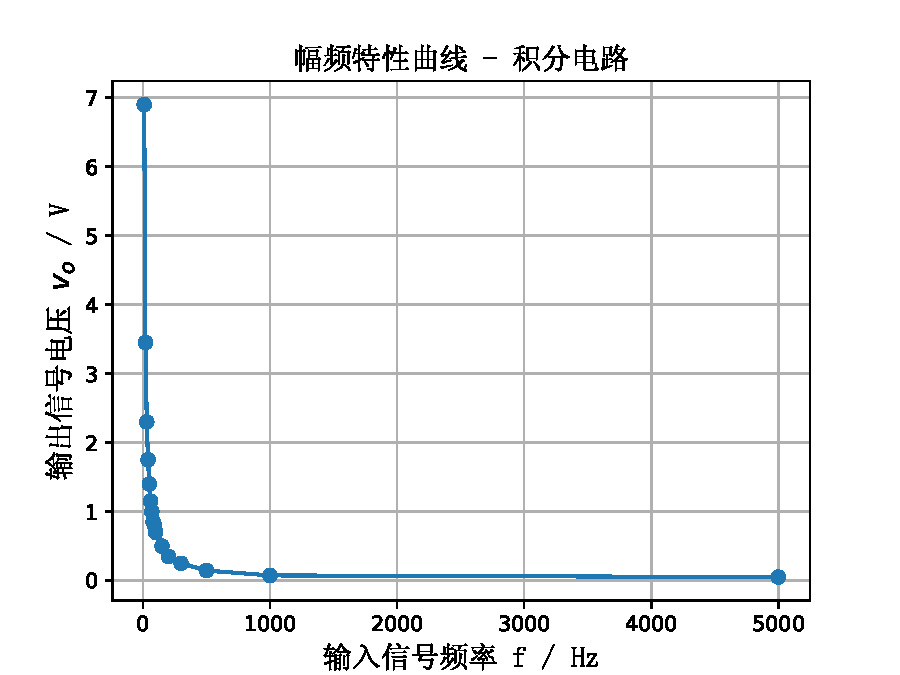
\includegraphics[width=10cm]{fig/AFC_int.pdf}\\
\caption{积分电路的幅频特性曲线}\label{AFC_int_fig}
\end{figure}
\subsubsection{方波输入波形图}
取输入信号为方波时,输入输出波形如图(\ref{20Hz_int_s})、(\ref{1kHz_int_s})、(\ref{2kHz_int_s}):
\begin{figure}[!h]
\centering
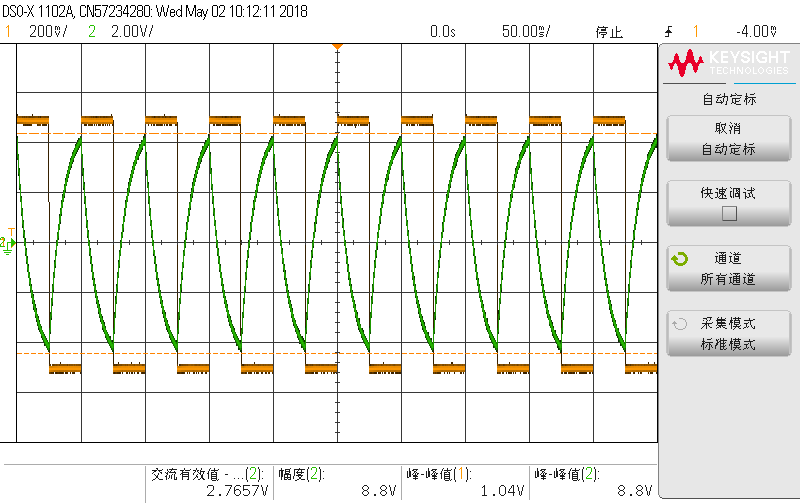
\includegraphics[width=8cm]{fig/scope_1.png}\\
\caption{改进的积分电路,方波输入,20Hz}\label{20Hz_int_s}
\end{figure}
\begin{figure}[!h]
\centering
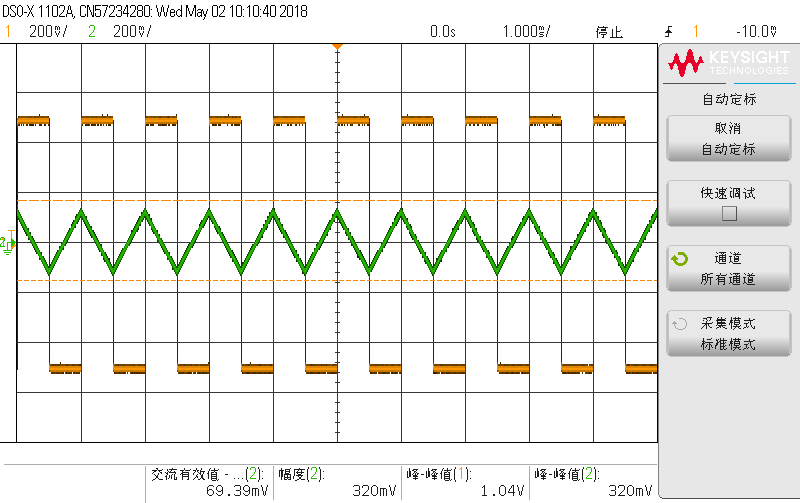
\includegraphics[width=8cm]{fig/scope_2.png}\\
\caption{改进的积分电路,方波输入,1kHz}\label{1kHz_int_s}
\end{figure}
\begin{figure}[!h]
\centering
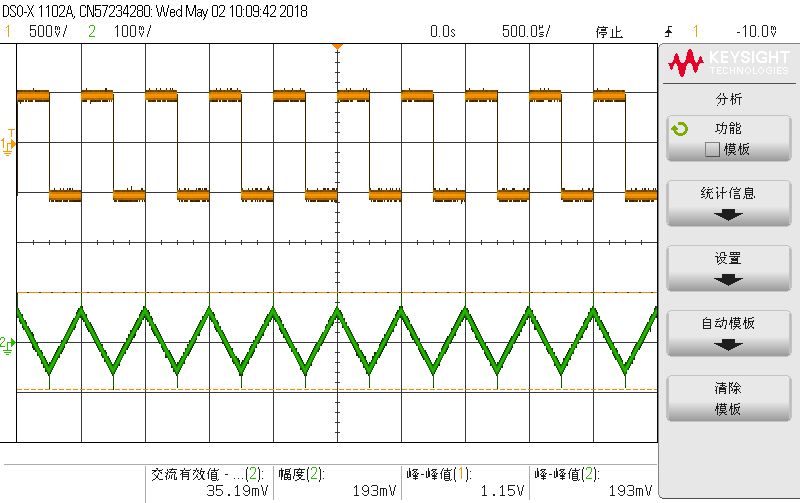
\includegraphics[width=8cm]{fig/scope_3.png}\\
\caption{改进的积分电路,方波输入,2kHz}\label{2kHz_int_s}
\end{figure}
\newpage
\subsection{微分电路}
图(\ref{diffcd_s})中的电阻为$R_2$=155.328$\Omega$。
\subsubsection{微分电路幅频特性}
微分电路的幅频特性数据如表(\ref{diff_AFC_table}):
\begin{table}[!h]
\centering
\caption{微分电路幅频响应}
\label{diff_AFC_table}
\begin{tabular}{|c|c|c|c|c|c|c|c|c|c|}
\hline
\rowcolor[HTML]{EFEFEF} 
$f_i$/Hz                     & 5      & 6      & 7     & 8      & 9      & 10     & 20     & 30    & 40     \\ \hline
$v_o(V_{PP})$/V              & 0.037  & 0.044  & 0.050 & 0.058  & 0.065  & 0.071  & 0.143  & 0.212 & 0.283  \\ \hline
$v_o(幅值=\frac{V_{PP}}{2})$/V & 0.0185 & 0.022  & 0.025 & 0.029  & 0.0345 & 0.0355 & 0.0725 & 0.106 & 0.1425 \\ \hline
\rowcolor[HTML]{EFEFEF} 
$f_i$/Hz                     & 50     & 60     & 70    & 71     & 80     & 90     & 100    & 143   & 150    \\ \hline
$v_o(V_{PP})$/V              & 0.354  & 0.423  & 0.492 & 0.501  & 0.562  & 0.630  & 0.700  & 1.00  & 1.05   \\ \hline
$v_o(幅值=\frac{V_{PP}}{2})$/V & 0.177  & 0.2115 & 0.246 & 0.2505 & 0.281  & 0.315  & 0.35   & 0.5   & 0.5025 \\ \hline
\rowcolor[HTML]{EFEFEF} 
$f_i$/Hz                     & 200    & 300    & 500   & 1000   & 1520   & 2000   & 3000   & 4000  & 5000   \\ \hline
$v_o(V_{PP})$/V              & 1.4    & 2.1    & 3.47  & 6.8    & 10.0   & 12.7   & 17.6   & 21.8  & 21.3   \\ \hline
$v_o(幅值=\frac{V_{PP}}{2})$/V & 0.7    & 1.05   & 1.735 & 3.4    & 5.0    & 6.35   & 8.8    & 10.9  & 10.65  \\ \hline
\end{tabular}
\end{table}

根据表(\ref{int_AFC_table})画出幅频特性曲线,如图(\ref{AFC_int_fig}):
\begin{figure}[!h]
\centering
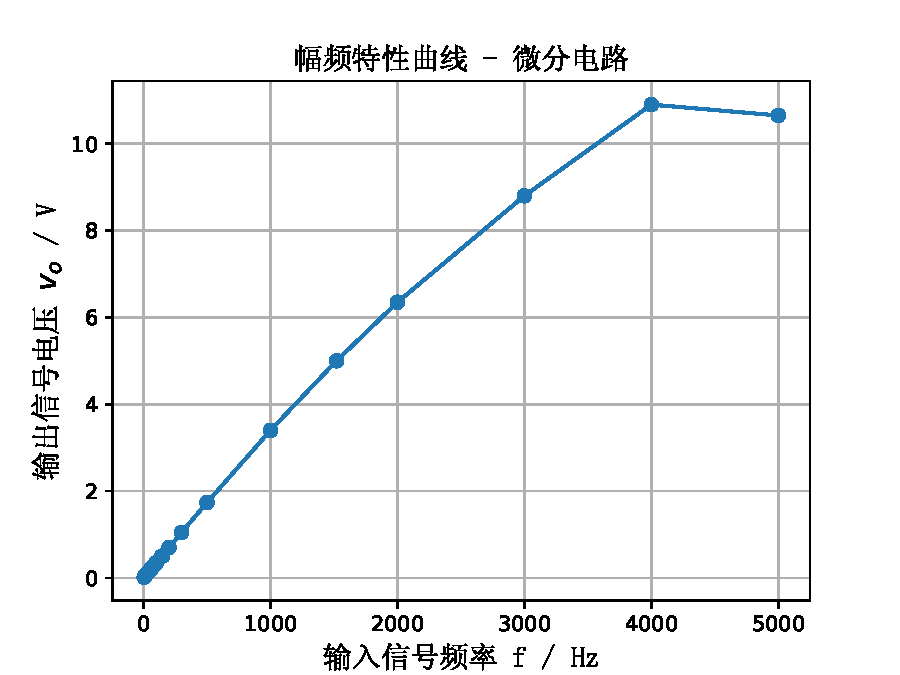
\includegraphics[width=10cm]{fig/AFC_diff.pdf}\\
\caption{微分电路的幅频特性曲线}\label{AFC_diff_fig}
\end{figure}
\subsubsection{方波输入波形图}
取输入信号为方波时,输入输出波形如图(\ref{10Hz_diff_s})、(\ref{100Hz_diff_s})、(\ref{1kHz_diff_s}):
\begin{figure}[!h]
\centering
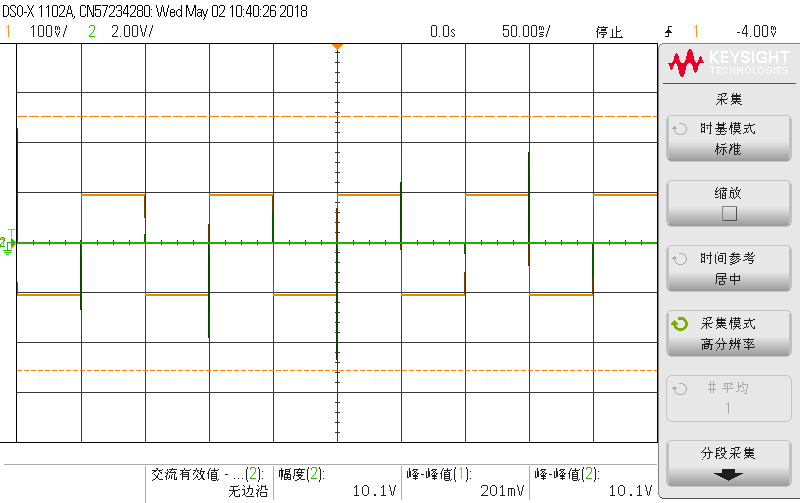
\includegraphics[width=8cm]{fig/scope_7.png}\\
\caption{改进的微分电路,方波输入,10Hz}\label{10Hz_diff_s}
\end{figure}
\begin{figure}[!h]
\centering
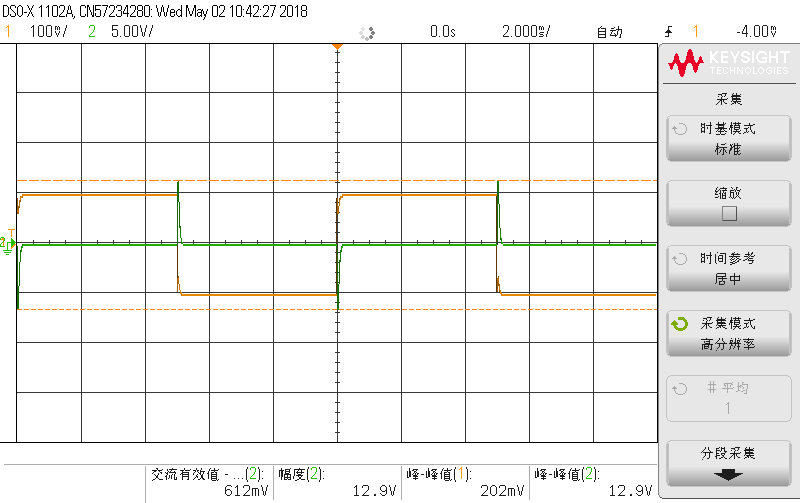
\includegraphics[width=8cm]{fig/scope_8.png}\\
\caption{改进的微分电路,方波输入,100Hz}\label{100Hz_diff_s}
\end{figure}
\begin{figure}[!h]
\centering
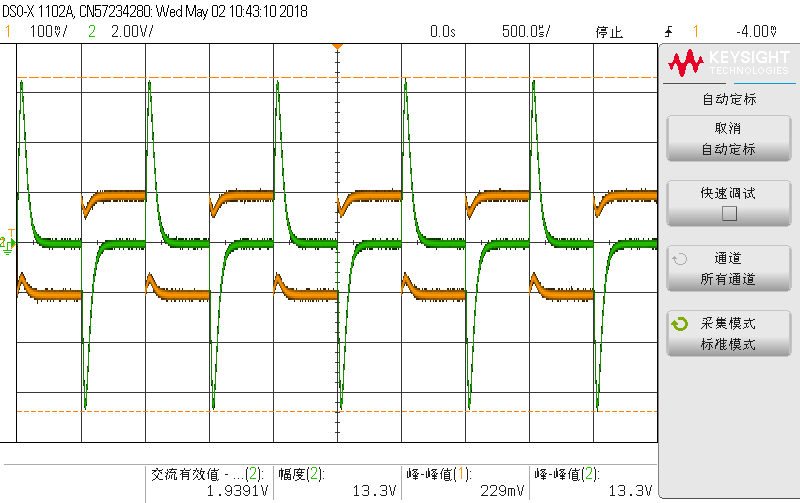
\includegraphics[width=8cm]{fig/scope_9.png}\\
\caption{改进的微分电路,方波输入,1kHz}\label{1kHz_diff_s}
\end{figure}

\subsection{积分-微分电路}
积分微分电路的幅频特性数据如表(\ref{int-diff-table}):
\begin{table}[!h]
\centering
\caption{积分-微分电路幅频响应}
\label{int-diff-table}
\begin{tabular}{|c|c|c|c|c|c|c|c|c|c|}
\hline
\rowcolor[HTML]{EFEFEF} 
$f_i$/kHz    & 0.01 & 0.02 & 0.05 & 0.1  & 0.2  & 0.5   & 1     & 2     & 3     \\ \hline
$v_{opp}$/mV & 5.6  & 5.8  & 9.1  & 10.1 & 10.2 & 10.8  & 11.8  & 13.6  & 15.25 \\ \hline
\rowcolor[HTML]{EFEFEF} 
$f_i$/kHz    & 4    & 4.5  & 5    & 5.5  & 6    & 6.2   & 6.4   & 6.6   & 6.8   \\ \hline
$v_{opp}$/mV & 17.8 & 23.5 & 28   & 38   & 56   & 68    & 86    & 122.5 & 202.5 \\ \hline
\rowcolor[HTML]{EFEFEF} 
$f_i$/kHz    & 6.9  & 7    & 7.1  & 7.2  & 7.3  & 7.4   & 7.6   & 7.8   & 8     \\ \hline
$v_{opp}$/mV & 295  & 500  & 790  & 470  & 285  & 205   & 130   & 96    & 76    \\ \hline
\rowcolor[HTML]{EFEFEF} 
$f_i$/kHz    & 8.2  & 8.5  & 9    & 9.5  & 10   & 15    & 20    & 50    &       \\ \hline
$v_{opp}$/mV & 65   & 53   & 41   & 35.5 & 30   & 17.25 & 15.25 & 11.8  &       \\ \hline
\end{tabular}
\end{table}

将其画图可得图(\ref{AFC_int_diff_fig}):
\begin{figure}[!h]
\centering
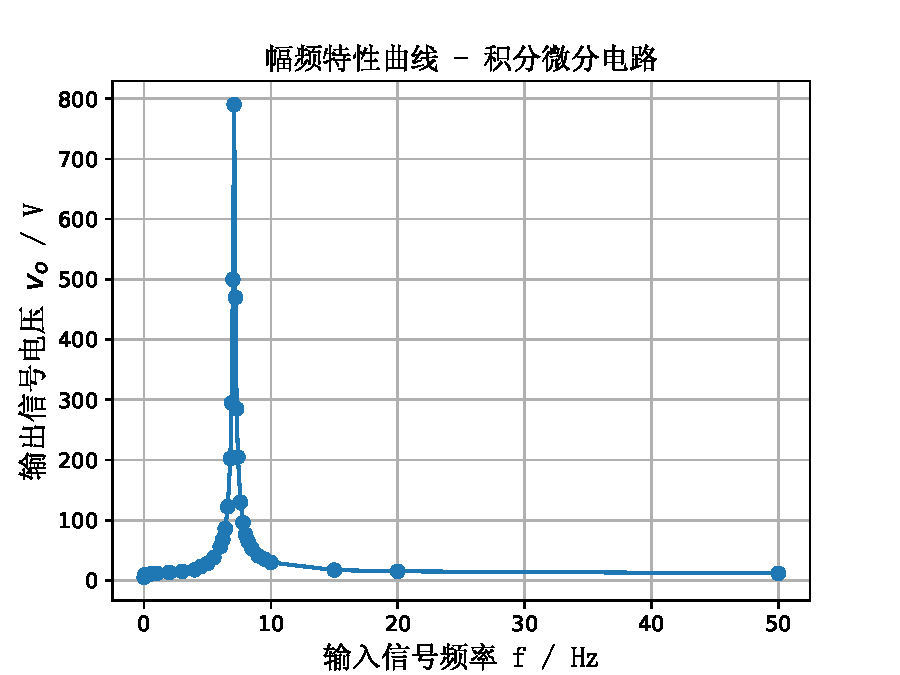
\includegraphics[width=12cm]{fig/AFC_int_diff.pdf}\\
\caption{积分微分电路幅频特性曲线}\label{AFC_int_diff_fig}
\end{figure}

根据图(\ref{AFC_int_diff_fig})可明显观察到所谓“小刺”,即幅频特性曲线中一个突起的峰。

\section{实验讨论与误差分析}
\begin{enumerate}
\item 测量准确性\\
在测量积分电路幅频特性数据时,当输出电压很小时,示波器显示的波形及其不清晰,其测量功能测到的数据波动极大。因此测得的数据可能不准确。
\item 不接电阻$R_2$时积分电路的幅频特性\\
接了电阻$R_2$时,积分电路在低频下的波形图如图(\ref{20Hz_int_s}),可以看到输出信号的三角波明显发生了弯曲。在不接电阻$R_2$时,测得低频下的波形图如图(bxt4):
\begin{figure}[!h]
\centering
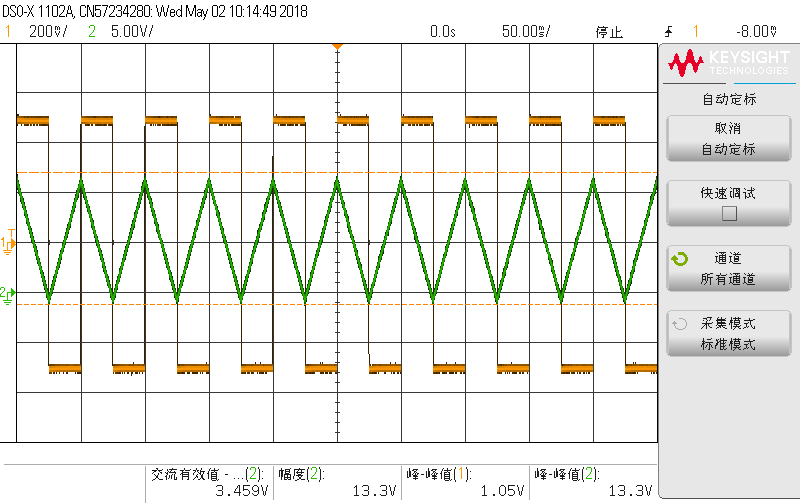
\includegraphics[width=8cm]{fig/scope_4.png}\\
\caption{使用图(\ref{intcd}),方波输入,20Hz}\label{bxt4}
\end{figure}

可以看到输出三角波的形状十分良好。
\end{enumerate}

\section{思考题}
\begin{enumerate}
\item \textbf{在图(\ref{intcd})中,若出现了较大的直流漂移,在电容两端并联一个100k$\Omega$的电阻可基本抑制直流漂移,试述其原因。}\\
通过查阅资料$^{\cite{zhidao}}$得知,如果没有这个电阻,电路是交流反馈,交流反馈可以改变电路参数,但由于电容的隔直,无法抑制缓慢变化的直流漂移。通过并联一个电阻,在电路中引入了直流反馈,从而能抑制直流信号变化,抑制零点漂移。
\item \textbf{图(\ref{int-diff-cd})中,若改选$R_1$=10$\Omega$,$C_1$=100$\mu$F,$R_1$与$C_1$乘积不变,这样是否可以?为什么?}\\
不可以。根据实验书中式(1-6-3):
\begin{equation}
H_{I1} = \cfrac{V_o(s)}{V_i(o)} = -\cfrac{R_2}{R_1}\cfrac{1}{R_2C_s+1}\label{1-6-3}
\end{equation}
可知,若将$R_1$由10k$\Omega$改为10$\Omega$,该电路对输入直流失调电压放大了10000倍,这将对电路产生较大影响。
\item \textbf{若加了155$\Omega$电阻的图(\ref{int-diff-cd})中的运放为理想运放,试用EWB仿真有无$R_2$时的幅频特性曲线。试述产生差别的原因。}\\
进行EWB仿真的结果如图(\ref{EWB})所示:
\begin{figure}[!h]
\centering
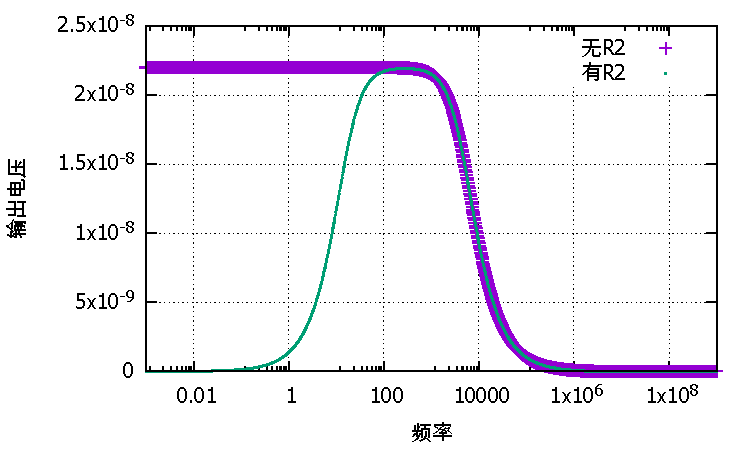
\includegraphics[width=9cm]{fig/question4.pdf}\\
\caption{EWB仿真幅频特性曲线}\label{EWB}
\end{figure}

从图中可以看出,没有$R_2$时,其幅频特性曲线在低频时几乎没有变化,即可以认为是直流放大。
\end{enumerate}

\nocite{jiaocai}
%--------bib------------------
\bibliography{ref}
\end{document}